\documentclass[10pt]{article}
\usepackage[english]{babel}
\usepackage[utf8]{inputenc}
\usepackage{amsmath}
\usepackage{amsfonts}
\usepackage{graphicx}
\usepackage[colorinlistoftodos]{todonotes}

\title{Progress report: \\
	Repair probabilities for the RCL polymer with two DSBs}
\author{Ignacio Madrid}

\begin{document}

\maketitle

\section{Motivation}


\section{Methods}
 To simulate the chromatin repair, we consider the model of a randomly cross-linked (RCL) polymer. A RCL polymer is formed by a classical Rouse chain of $N$ monomers as backbone and $N_c$ extra random cross-links which are added uniformly over all combinations of non-neighbor monomer pairs. We define the RCL polymer connectivity $\xi$ as the fraction of added cross-links with respect to the total number of possible pairings, i.e. $\xi = Nc/((N-1)(N-2)/2)$. 
 
 We define two admittance (Laplacian) matrices that characterize the RCL polymer: the Rouse matrix $M$ which describes the backbone adjacency, and $B$ which describe the added connectors.

  
 The model simulated is described in figure \ref{fig:model}.

  We supposed the RCL polymer subdued to Langevin dynamics, i.e., if the monomer positions of the polymer in time are represented by $(R_t)_{t\geq0} = (R_1, ..., R_N)_{t\geq0}$ with $R_i \in \mathbb{R}^3, i = 1,...,N$, the dynamics are described by the equation:
 
 $$ dR_t = -\frac{1}{\zeta} \nabla \phi(R_t) dt + \sqrt{2D} dW_t $$
 
 where $\zeta$ is the friction coefficient, $\phi$ is an harmonic potential, $D$ is the diffusion coefficient and $(W_t)_{t \geq 0}$ is a $N \times 3$-dimensional Brownian motion. 
 
 The harmonic potential of an RCL polymer is given by the classical Rouse potential and by the potential induced by the random cross-links:
 
 $$
 \phi(R) = \frac{\kappa}{2} \sum_{n = 1}^{N-1} ||R_{n+1} - R_{n}||^2 + \frac{\kappa'}{2} \sum_{i,j \in \mathcal{R}} ||R_{i} - R_{j}||^2 =\frac{\kappa}{2} \text{tr}(R^TMR) + \frac{\kappa'}{2} \text{tr}(R^TBR) $$

 where $\kappa$ and $\kappa' $ are spring constants we will suppose equal,  $M$ is the Rouse matrix (degree - connectivity), $B$ is the degree - connectivity matrix with the added random connectors, and $\mathcal{R}$ is the set of monomers which have been randomly connected. Since $\frac{\kappa}{\gamma} = \frac{3D}{b^2}$ where $b$ is the standard deviation of the bonds length, we'll consider the equation :
 
 $$
 dR_t = -\frac{3D}{b^2} (M + B) R_t dt + \sqrt{2D} dW_t
 $$
 
 In the following, we implement the Euler's scheme of the previous equation setting $D = 0.008 \ \mu^2$m/s and $b = 0.2 \ \mu$m . In particular, we are interested on the probability of repair after two random breaks (in monomers $A_1 - A_2, B_1 - B_2$, where $A_1 \sim \mathcal{U}[1,N-g-2], \ 1 \leq A_1 < A_2 = A_1 + 1 < B_1 < B_2 = B_1 + 1 < N$) with a deterministic inter-break genomic distance $g$ between them ($B_1 - A_2 = g$).
 
 So, if we define the first encounter time as
$$
T_{m,n}^{\epsilon} := \inf \{ t \geq 0 : ||(R_m)_t - (R_n)_t|| < \epsilon  \}
$$
where $R_m$ and $R_n$ are the positions of monomers $m$ and $n$, and $\epsilon$ is the encounter distance, then the repair probability is
$$
\mathbb{P}(Repair) = \mathbb{P}(T_{A_1,A_2}^\epsilon \wedge T_{A_1,A_2}^\epsilon \leq T_{A_1,B_1}^\epsilon \wedge T_{A_1,B_2}^\epsilon \wedge T_{A_2,B_1}^\epsilon \wedge T_{A_2,B_2}^\epsilon )
$$

NB: By pure chance, the expected repair probability is $2/6 = 1/3$.

\begin{figure}[!h]
\centering
\includegraphics[width=\textwidth]{../drawings/modele.png}
\caption{Model of an RCL polymer for chromatin repair simulations. Two random breaks are induced with a deterministic inter-break genomic distance between them. Random cross-links are built uniformly over all combinations of non-neighbor monomers. In the break moment, the cross-links in damage foci (e.g. the CL in monomer $B_2$) might be removed along with the broken bonds. Excluded volume interactions can also be added in the form of a repulsive harmonic potential in the disconnected monomers, simulating the reported chromatin expansion induced just after the DSBs. Finally, repair occurs when two separated neighbors meet at a distance inferior to an encounter distance $\varepsilon$.}
\label{fig:model}
\end{figure}

\clearpage

\section{Results}

\subsection{First Encounter Time (FET) distribution}

Since an important peak was observed at instant 0 in the first simulations, we decided to wait some time after the induction of double strand breaks (DSBs), before measuring if any pair of monomers have encountered. 
Concerning the encounters events, if two or more pairs of monomers encounter at the same simulated instant, we toss a coin to choose uniformly over those pairs to be the first encounter.

\begin{figure}[h!]
	\centering
	\includegraphics[width=\textwidth]{../DNA_Religation/figures/FEThistograms_keepingANDremoving.png}
	\caption{Distribution of the first encounter time keeping and removing the cross-links in the cleaved monomers. An exponential distribution has been fitted to each histogram. The results corresponds to a polymer of 100 monomers, 5 random cross-links, with two DSBs at a genomic distance of 10 and a waiting after-break time of 25 seconds. The events which take longer than 60 seconds are ignored.}
	\label{fig:hists}
\end{figure}

The results of figure \ref{fig:hists} indicate that the removal of cross-links does not seem to affect the mean first encounter time, nor the ratio of misrepair/repair events. The estimated rate parameter ($\lambda$) is 0.08 for both cases. It should be noted that since the maximum time of simulation is set at 60 seconds (i.e. if nothing happens in 60 seconds the simulation is discarded) the distribution is biased and corresponds to $\mathcal{L}(FET|FET<60)$. For instance, when the simulation maximum time has been increased to 200 seconds, the rate parameter is estimated at 0.04.


%Finally as we see in figure \ref{fig:hists2} within the misrepair events, the mismatchs seems to be equidistributed. 

\begin{figure}[h!]
	\centering
	\includegraphics[width=\textwidth]{../DNA_Religation/figures/eventsRepartition.png}
	\caption{Distribution of the first encounter time keeping the CLs in the damage foci, and distribution of the repair and misrepair events (1000 realisations).}
	\label{fig:hists2}
\end{figure}

\newpage

\subsection{Repair probability}

\subsubsection{Effect of the genomic distance between two DSBs}

\begin{figure}[h]
	\centering
	\includegraphics[width=\textwidth]{../DNA_Religation/projects/RCLPolymer_Repair_Probability/Figures/proba_v_g__100monomers_keepingandremovingCLs.png}
	\caption{Repair probability against the genomic distance between the two DSBs. Polymer of 100 monomers with 15 random cross-links. Encounter distance of 0.1 $\mu$m (and b = 0.2 $\mu$m).}
	\label{fig:proba_v_g_1}
\end{figure}

We see in figure \ref{fig:proba_v_g_1} that regardless the removal of cross-links the repair probability increases in the same way as the inter-break genomic distance increases. So, removing the cross-links in the disconnected monomers does not seem to induce a better repair probability

\begin{figure}[h]
	\centering
	\includegraphics[width=0.7\textwidth]{../DNA_Religation/projects/RCLPolymer_Repair_Probability/Figures/proba_v_g__keepingCLs.png}
	\caption{Repair probability against the genomic distance between the two DSBs. Polymer of 100 monomers with 10 random cross-links. Encounter distance of 0.1 $\mu$m (and b = 0.2 $\mu$m).}
	\label{fig:proba_v_g_2}
\end{figure}

The most interesting remark though is the gap between the probabilities at a genomic distance of 1 (i.e. the two DSBs are connected, $A2$ and $B1$ being neighbors) and the other genomic distances (figure \ref{fig:proba_v_g_2}). As only valid cuts are allowed (i.e. the polymer rests fully connected after the breaks) the segment $A_2-B_1$ is indeed connected to the upstream and/or the downstream fragment. The probability of being connected to only one of them is higher than the probability of being connected to both, so the segment could be pushed towards one of the free monomers rapidly and then induce a good ratio of repair.

\subsubsection{Effect of the number of cross-links}

\begin{figure}[h!]
	\centering
	\includegraphics[width=\textwidth]{../DNA_Religation/projects/RCLPolymer_Repair_Probability/Figures/proba_v_Nc__100monomers_01eps_removingCLs_500iteration_goodDT.png}
	\caption{Polymer of 100 monomers. Repair probability against the number of random cross-links when removing the random CLs in damage foci.}
	\label{fig:proba_v_cl}
\end{figure}

Increasing the number of cross-links approaches the simulated probabilities to $1/3$, which is the result expected by pure chance. Indeed, increasing the number of CLs and therefore approaching all monomers not only increases the chances of a good matching, but also the bad match case. It is interesting that systems which had a repair probability $\leq 1/3$  because had DSBs at a small genomic distance (so the chances of a bad matching where higher) improve their repair probabilities when we increase the number of cross-links. In other words, \textbf{the compactness may help to repair polymers cut in a small neighborhood.}

In effect, increasing the number of random connectors increases as well the compactness of the polymer, revealed as a decrease of the mean radius of gyration (cf. figure \ref{fig:mrg_v_nc}). Besides, we can see that the position of the breaks does not affect the ensemble mean of the gyration radius.

\begin{figure}[h!]
	\centering
	\includegraphics[width=\textwidth]{../DNA_Religation/projects/RCLPolymer_Repair_Probability/Figures/MRG_vs_CLnumber_3genomicdistances.png}
	\caption{Polymer of 100 monomers. Mean radius of gyration in function of the number of cross-links.}
	\label{fig:mrg_v_nc}
\end{figure}
  


\subsubsection{Effect of Excluded Volume}

Excluded volume interactions to simulate self-avoidance are added to the polymer dynamics through a new harmonic potential that is added to the potential considered in the Langevin equation:

$$
\phi_{ev}(R) = - \frac{\kappa_{ev}}{2} \sum_{i,j \ : \ i \neq j} ||R_i - R_j ||^2 1_{||R_i - R_j || < \sigma}
$$

In practice, to simulate the dispersion of chromatin in the break region, we induce volume exclusion to the damage foci monomers only and take $\kappa_{ev} = \kappa$:

$$
\phi_{local-ev}(R) = - \frac{\kappa_{ev}}{2} \sum_{i \in \text{Damage foci}}\sum_{j \neq i} ||R_i - R_j ||^2 1_{||R_i - R_j || < \sigma}
$$

$\sigma$ is a cutoff radius for the excluded volume interactions. Larger values of $\sigma$ make the waiting for looping times last longer (figure \ref{fig:mFET_v_Nc_EV}) and thus make the encounter events rarer, however they do not affect dramatically the repair probability overall (figure \ref{fig:vs_volumeexclusionradius}). 


\begin{figure}[h]
	\centering
	\includegraphics[width=\textwidth]{../DNA_Religation/projects/RCLPolymer_ExcludedVolumeExperiments/figures/meanFET_vs_VE_Nc.png}
	\caption{Mean first encounter times in function of the number of cross-links, with and without a radius of 0.1 $\mu$m of excluded volume in the damage zone.}
	\label{fig:mFET_v_Nc_EV}
\end{figure}

\begin{figure}[h]
	\centering
	\includegraphics[width=\textwidth]{../DNA_Religation/projects/RCLPolymer_ExcludedVolumeExperiments/figures/proba_vs_cutoffradius_goodone.png}
	\caption{Probability and 95\% confidence interval of repair, in function of the cutoff radius of volume exclusion.}
	\label{fig:vs_volumeexclusionradius}
\end{figure}

We see in figure \ref{fig:MSRGandFET_byEvent} that, as expected, the misrepair scenarios are associated with smaller radius of gyration, and thus with more compact polymers. This could be an indication that relaxation of the polymer chain in the damage loci could lead to better repair probabilities. 

\begin{figure}[h]
	\centering
	\includegraphics[width=\textwidth]{../DNA_Religation/projects/RCLPolymer_Repair_Probability/figures/by_event_type_distributions.png}
	\caption{Distribution of the first encounter times and the mean square radius of gyration in repair and misrepair events considering local excluded volume interactions.}
	\label{fig:MSRGandFET_byEvent}
\end{figure}

We can see in figure \ref{fig:pr_v_g_cutoffs} that the repair probability in function of the genomic separation between the breaks behaves similarly that previously (cf. figure \ref{fig:proba_v_g_1}). 

\begin{figure}[h]
	\centering
	\includegraphics[width=\textwidth]{../DNA_Religation/projects/RCLPolymer_Repair_Probability/figures/proba_v_g_VEcutoffs.png}
	\caption{Probability and 95\% confidence interval of repair, in function of interbreak genomic distance for exclusion cutoffs  $b/2$ and $b$ ($b = 0.1 \mu$m).}
	\label{fig:pr_v_g_cutoffs}
\end{figure}

Surprisingly however the repair probability function considering excluded volume interactions is always below the repair probability in the non-excluded case (figures \ref{fig:proba_vs_g_exclusion} and \ref{fig:proba_vs_Nc_exclusion})

\begin{figure}[h]
	\centering
	\includegraphics[width=\textwidth]{../DNA_Religation/projects/RCLPolymer_ExcludedVolumeExperiments/figures/proba_vs_genomicDistance_excludedANDnot_01cutoff.png}
	\caption{Probability of repair in function of the genomic separation between the breaks.}
	\label{fig:proba_vs_g_exclusion}
\end{figure}

\begin{figure}[h]
	\centering
	\includegraphics[width=\textwidth]{../DNA_Religation/projects/RCLPolymer_ExcludedVolumeExperiments/figures/proba_v_Nc.png}
	\caption{Probability of repair in function of the number of random cross-links, for two breaks separated by 4 monomers (g=5).}
	\label{fig:proba_vs_Nc_exclusion}
\end{figure}

\begin{figure}[h]
	\centering
	\includegraphics[width=\textwidth]{../DNA_Religation/projects/RCLPolymer_ExcludedVolumeExperiments/figures/proba_v_g_EV_03_20Nc}
	\caption{Probability of repair in function of the genomic separation between the breaks. Even for small genomic distances and high connectivity (20 random cross-links) the local volume exclusion seems to interfere with the correct repair, rather than helping it.}
	\label{fig:proba_vs_g_03exclusion}
\end{figure}

\begin{figure}[h]
	\centering
	\includegraphics[width=\textwidth]{../DNA_Religation/projects/RCLPolymer_ExcludedVolumeExperiments/figures/proba_v_Nc_EV_03_4g}
	\caption{Probability of repair in function of the total number of cross-links, with an inter-break genomic distance $g = 4$. }
	\label{fig:proba_vs_Nc_03exclusion}
\end{figure}


\clearpage

\subsubsection{Effect of volume exclusion with more restrictive encounter distances}

After tracking the inter-break physical distances (in $\mu$m) as it is presented in figure \ref{fig:distances3breaks}, it seems that the encounter distance of 0.1 $\mu$m is rather permissive. So, smaller encounter radius will be considered now to see if excluded volume could help the correct repairs.

\begin{figure}[h]
	\centering
	\includegraphics[width=\textwidth]{../DNA_Religation/projects/DSB_Clustering/figures/distanceBetween3DSBs}
	\caption{Track of the distances between the ends of three DSBs just before the breaks are induced at relaxation time. The ends of the same break tend to be nearer in comparison to the other distances. }
	\label{fig:distances3breaks}
\end{figure}

Figure \ref{fig:noExclusion_002epsilon} shows the results with and without volume exclusion and with a encounter distance of $\varepsilon = b \cdot 10^{-1} = 0.02 \mu$m.

\begin{figure}[h]
	\centering
	\includegraphics[width=\textwidth]{../DNA_Religation/figures/eventsandFET_002epsilon_VE}
	\caption{Encounter results with and without volume exclusion for a two DSBs at a genomic distance of 4 and considering 20 random cross-links. \textbf{a}. Experiment set. \textbf{a}. Encounter events distribution. The most frequent mismatch corresponds to the looping of the central fragment of the broken polymer. \textbf{c}. First Encounter Time distribution of all the events. \textbf{d}. Same results considering volume exclusion with a cutoff radius of 0.1 $\mu$m.}
	\label{fig:noExclusion_002epsilon}
\end{figure}





\clearpage

\subsection{Repair probability in different domains}

We'll now consider a polymer replied in two connected sub-domains (TADs) (figure \ref{fig:TADSmodel}).

\begin{figure}[!h]
	\centering
	\includegraphics[width=\textwidth]{../drawings/twoTADmodel.png}
	\caption{Model of the RCL polymer replied in two connected subdomains.}
	\label{fig:TADSmodel}
\end{figure}


Figure \ref{fig:proba_v_interTADdistance} shows the repair probabilities of two DSBs located at independent connected sub-domains. We see that the correct repair rate is visible higher. The probabilities are observed for two sub-domains where the genomic distance that separate them is increased. The distance between the two sub-domains does not seem to affect the (already good) probability of correct repair. 

The following figures illustrates the following experiment: two DSBs are induced \textbf{in the same sub-domain} with a genomic distance between the breaks as in the previous section. The repair probability is measured again to see if the presence of a juxtaposed sub-domain without breaks affects the repair in the first sub-domain.


\begin{figure}[h]
	\centering
	\includegraphics[width=0.7\textwidth]{../DNA_Religation/projects/RCLPolymer_TwoDomains/figures/RepairProba_v_interTADdistance.png}
	\caption{One DSB in each subdomain (two subdomains of size 50). Repair probability vs. inter-TAD separation distance.}
	\label{fig:proba_v_interTADdistance}
\end{figure}


\begin{figure}[h]
	\centering
	\includegraphics[width=0.7\textwidth]{proba_v_g_2domains.png}
	\caption{Probability and 95\% confidence interval of repair, in function of the interbreak distance for two DSBs induced in one sub-domain of size 100 on a polymer formed by two sub-domains (100 and 50 monomers). The subdomain had 5 RCLs.}
	\label{fig:2domain}
\end{figure}



\begin{figure}[h]
	\centering
	\includegraphics[width=0.7\textwidth]{../DNA_Religation/projects/RCLPolymer_TwoDomains/figures/proba_v_g_2domains_10randomconnectors}
	\caption{Probability and 95\% confidence interval of repair, in function of the interbreak distance for two DSBs induced in one sub-domain of size 100 on a polymer formed by two sub-domains (100 and 50 monomers). The subdomain had 10 RCLs.}
	\label{fig:2domain_10rcls}
\end{figure}


\clearpage


\begin{figure}[h]
	\centering
	\includegraphics[width=0.7\textwidth]{../DNA_Religation/projects/RCLPolymer_TwoDomains/figures/proba_vs_longrange_first}
	\caption{Probability of repair in function of the number of long-range connectors. Two DSBs were induced at a genomic distance of 5 in the first sub-domain of a polymer conformed by 2 sub-domains of 100 monomers with 10 inner cross-links.}
	\label{fig:proba_v_longrange}
\end{figure}

Figures \ref{fig:proba_v_parasytes} and \ref{fig:proba_v_longrange_sizes} suggest that the presence of a juxtaposed cross-linked polymer chain of any size does not affect the repair performance for two DSBs at a given genomic distance when the number of long-range connectors remains little. Figure \ref{fig:proba_v_longrange_3and45} suggest that a higher number of long-range connectors increases the randomness of the system, making the probabilities go to $1/3$. If the correct repair probability was already about $1/3$ without long-range connections (for example, thanks to a high number of intra-domain cross-links), adding the long-range links does not change the repair rates.

\begin{figure}[h]
	\centering
	\includegraphics[width=\textwidth]{../DNA_Religation/projects/RCLPolymer_TwoDomains/figures/proba_vs_genomicdistance_parasytes}
	\caption{Repair probability of a 100-monomers sub-domain with two DSBs, in function of the genomic inter-break distance between the DSBs. Juxtaposed to the broken sub-domain, there is another sub-domain of size 50, 100 and 200 without breaks. The first sub-domain has 10 inner cross-links and the juxtaposed one has a connectivity of 0.2\%. There are no long-range connectors between the two sub-domains.}
	\label{fig:proba_v_parasytes}
\end{figure}

\begin{figure}[h]
	\centering
	\includegraphics[width=\textwidth]{../DNA_Religation/projects/RCLPolymer_TwoDomains/figures/proba_v_longrangeNum_3AND45}
	\caption{Probability of repair in function of the number of long-range connectors. Two DSBs were induced at a genomic distance of 5 in the first sub-domain of a polymer conformed by 2 sub-domains of 100 monomers with 3 and 45 inner cross-links.}
	\label{fig:proba_v_longrange_3and45}
\end{figure}

\begin{figure}[h]
	\centering
	\includegraphics[width=\textwidth]{../DNA_Religation/projects/RCLPolymer_TwoDomains/figures/proba_v_longrangeNum_differentsizes}
	\caption{Probability of repair for 0,2,4 and 6 long-range connectors, and different sizes for the juxtaposed unbroken sub-domain. Two DSBs were induced at a genomic distance of 30 in the first sub-domain (100 monomers). The juxtaposed sub-domain has a constant connectivity fraction (0.2\%).}
	\label{fig:proba_v_longrange_sizes}
\end{figure}






\clearpage

\subsubsection{TODO}
\begin{itemize}
\item For one DSB in each TAD: Simulate the repair probability vs. intra-TAD connectors number
\item For one DSB in each TAD: Simulate the repair probability vs. long-range connectors number
\item For two DSB in a TAD: Compare repair probabilities with the results obtained in the previous section. Does a second TAD (with no breaks) affect the repair probability of the first one? How?
\end{itemize}

\clearpage

\section{Partial conclusions}
\begin{itemize}
	\item When the mismatch rate is high (near DSBs and/or high connectivity) the most common misrepair seems to be the $"a_2-b_1$" one, which corresponds to the looping of the central segment of the cut RCL polymer.
	\item Keeping or removing the cross-links in the separated neighbors does not seem to particularly help the repair, at least without considering volume exclusion. The joint action of CLs removal and volume exclusion in the damage foci should be analyzed more carefully to conclude if this "relaxation" helps or not the repair.
	\item If there are enough cross-links, even for DSBs separated by a large genomic distance the repair probability goes down to $1/3$, i.e. the expected value by pure chance. The best correct repair probabilities occur, as one could expect, at large interbreak genomic distances with few random cross-links. However, if the breaks are close and the repair probability is less than $1/3$, the increment of cross-links improves the correct match rate.
	\item Local excluded volume in the damage foci seems to do not affect or even obstruct the repair, rather than improving its probability. Probability curves with local local exclusion volume are indeed down shifted in comparison with the non-excluded ones.
\end{itemize}

\section{Perspectives}
\begin{itemize}
	\item Non-homologous end-joining repair : The repair probability curves in function of the inter-break genomic distance and the number of cross-links reveal a characteristic behavior (tendency to $1/3$ when the connectivity is high, a sort of logistic growth when the genomic distance between the breaks is increased) that could be verified analytically using the results available for the unbroken RCL polymer\footnote{O. Shukron and D. Holcman. Statistics of randomly cross-linked polymer models to interpret chromatin conformation capture data. \textbf{Phys. Rev. E} 2017 Jul:96, 012503}
	\item For the RCL polymer with subdomains : It has been reported that DSBs cluster. In particular, damaged active genes remain largely unrepaired and clustered to be repaired afterwards via homologous recombination in postreplicative cells\footnote{Aymard F. \textit{et al.} Genome-wide mapping of long-range contacts unveils clustering of DNA double-strand breaks at damaged active genes. \textbf{Nat Struct Mol Biol.} 2017 Apr;24(4):353-361}. It could be interesting to study if DSB clustering is a property inherent to the polymer dynamics, and if it is facilitated by exclude volume interactions and the local removal of cross-links in the damage foci.
\end{itemize}


\end{document}